\section{Object-Oriented Languages} 
\subsection{Single Inheritance of Data Fields}
单继承single-inheritance(SI): 每个类最多只能继承一个基类, 因此继承关系图是一棵树. 

\subsubsection{Field layout}
使用 *prefixing

\begin{figure}[H]
    \centering
    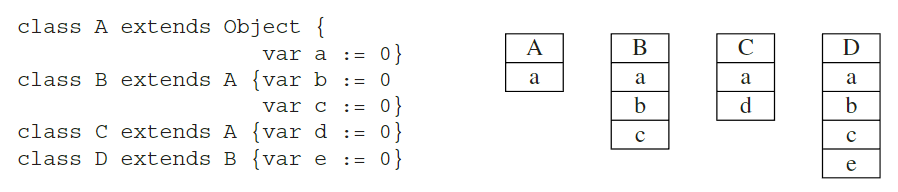
\includegraphics[width=0.84\linewidth]{pic/CP14/Single inheritance of data fields.}
    \caption{Single inheritance of data fields.}
\end{figure}
派生类新增的 fields 跟在基类的后面.

\subsubsection{Method dispatch}
每个 method 编译成一段代码(称为 method instance), 编译方式和普通函数几乎无异. 

每个类都对应一个 class decriptor, 里面包含了描述这个类的一些必要信息: 
\begin{itemize}
    \item 一个指向基类的指针
    \item 一个列表, 包含这个类所有的 method instances
\end{itemize}


对于 static method 的调用 $x.f()$, 编译器将会: 
\begin{enumerate}
    \item 找到对象 $x$ 对应的类, 记为 $C$.
    \item 如果 $C$ 中有 $f$, 则直接得出 $x.f()$ 翻译结果为 $C_f$; 否则继续向上(在基类中)寻找. 
    \item 假设 $C$ 的基类为 $B$, 在 $B$ 中查找 $f$, 如找到则得出 $x.f()$ 翻译结果为 $B_f$; 否则继续向上寻找. 
    \item $\dots$
    \item 直到在某个祖先中找到为止(或是一路找到Object还没有则报错), 调用它. 
\end{enumerate}

对于 dynamic method 的处理略复杂:
\begin{itemize}
    \item 每个类维护一个 dispatch vector (例如虚表 virtual methods table) 储存每个 method 的地址. 
    \subitem 建立方式类似 prefixing: 派生类中新声明的方法跟在基类 dispatch vector 的后面; 如果有基类的 method 被重写了, 也要替换成自己重写后 method 的地址. 
    \item 每个对象都关联某个 vtable: 对象的开头储存一个指针指向对应 class descriptor , 里面就有 vtable. 
    \item 需要动态查找(lookup), 有额外的开销. 
\end{itemize}

\begin{figure}[H]
    \centering
    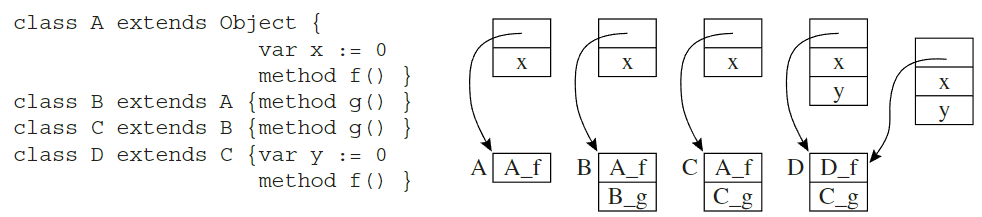
\includegraphics[width=0.84\linewidth]{pic/CP14/Class descriptors for dynamic method lookup}
    \caption{Class descriptors for dynamic method lookup}
\end{figure}

对于 dynamic method 的调用 $x.f()$, 编译器将会: 
\begin{enumerate}
    \item 在 $x$ 的 0 偏移处(开头)找到 class descriptor $d$.
    \item 由于方法 $f$ 的偏移量是确定的(记为 $F$), 从 $d$ 中 $F$ 偏移处获取 $f$ 的函数地址. 
    \item 调用f.
\end{enumerate}

\subsection{Multiple Inheritance of Data Fields}
多继承multiple-inheritance(MI): 每个类可以继承多个基类, 因此继承关系图是有向无环图(DAG).

\subsubsection{Field layout}
通过图染色获取. 

\begin{figure}[H]
    \centering
    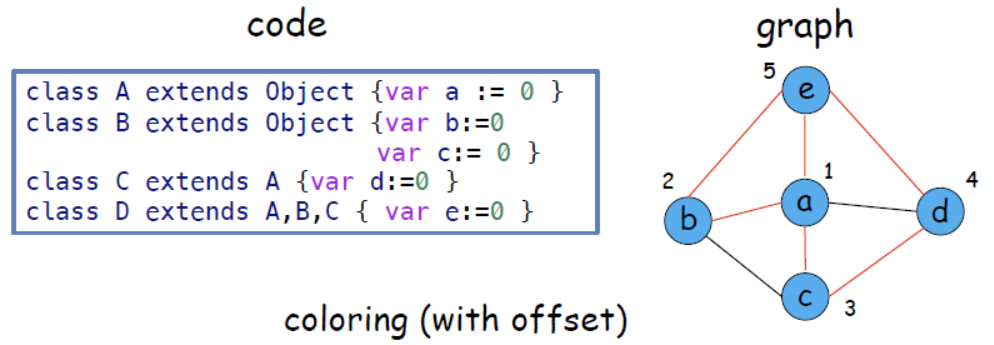
\includegraphics[width=0.84\linewidth]{pic/CP14/Multiple inheritance}
    \caption{Multiple inheritance}
    \label{fig:Multiple inheritance}
\end{figure}

目标: 静态分析所有类, 为每个 field 的找到一个固定偏移量. 如果不同 field 在同一个类中出现, 则不能共享同一个偏移量. 
\begin{itemize}
    \item 节点: 不同的 field 名
    \item 边: 同时在某个类中出现的 field 则连边
    \item 颜色: 最终偏移量(0, 1, 2, $\cdots$)
\end{itemize}

例如从 \textbf{Figure} \ref{fig:Multiple inheritance} 将得到 \textbf{Figure} \ref{fig:Multiple inheritance of data fields}.

\begin{figure}[H]
    \centering
    \begin{subfigure}{0.48\linewidth}
        \centering
        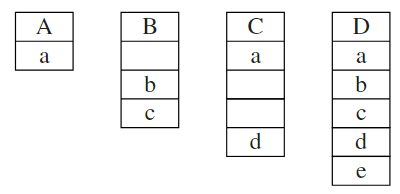
\includegraphics[width=\linewidth]{pic/CP14/Multiple inheritance of data fields}
        \caption{data fields}
        \label{fig:Multiple inheritance of data fields}
    \end{subfigure}
    \begin{subfigure}{0.48\linewidth}
        \centering
        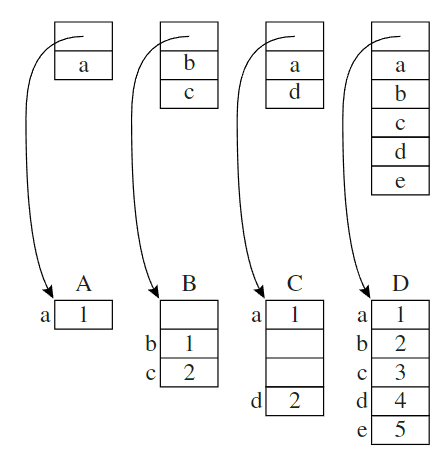
\includegraphics[width=0.65\linewidth]{pic/CP14/Field offsets in descriptors}
    \caption{Field offsets in descriptors}
    \label{fig:Field offsets in descriptors}
    \end{subfigure}
    \caption{Multiple inheritance}
\end{figure}


% \begin{figure}[H]
%     \centering
%     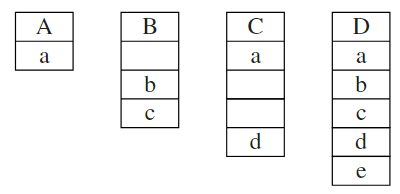
\includegraphics[width=0.618\linewidth]{pic/CP14/Multiple inheritance of data fields}
%     \caption{Multiple inheritance of data fields.}
%     \label{fig:Multiple inheritance of data fields}
% \end{figure}

% \begin{figure}[H]
%     \centering
%     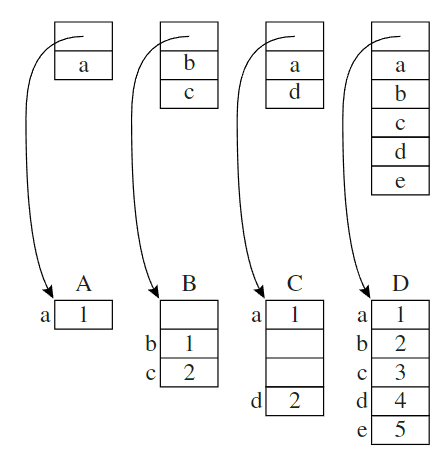
\includegraphics[width=0.44\linewidth]{pic/CP14/Field offsets in descriptors}
%     \caption{Field offsets in descriptors}
%     \label{fig:Field offsets in descriptors}
% \end{figure}

优化: 可以看出存在许多空的 slot 被浪费了. 我们可以把 fields 在内存上合并, 转而在每个类的 class descriptors 中记录各个 field 的真实偏移量. 如 \textbf{Figure} \ref{fig:Field offsets in descriptors} 所示. 



由于类的数量远少于对象(类的实例)数量, 所以这样能节省空间. 不过这种优化导致每个 field 的具体偏移不固定了, 因此需要在运行时在 class descriptor 中动态查找(lookup) field 的真实偏移量.

\subsubsection{Method dispatch}
仍然使用图染色. 直接把 method 名混合进上述的图中, 一起染色; 也就是不仅记录 field 的偏移量, 也记录 method 的地址. 也有动态查找的开销. 

解决方案: Hashing. 其实就是又包了一层新表, 允许通过 field/method 的名字本身索引到 field offset 或 method address. 更简单地说, 原先是 \mintinline{c++}{OffsetOrAddr[]} , 现在是 \mintinline{c++}{hashmap<Name, OffsetOrAddr>} .

\begin{itemize}
    \item Ftab(field table): field offset 或 method address
    \item Ktab(key-table): 记录注册过的名字
\end{itemize}

若要在 object $c$ 获取 field $b$, 编译器会:
\begin{enumerate}
    \item 在 $c$ 的 0 偏移处(开头)找到 class descriptor $d$.
    \item 从偏移量 $d+Ktab+hash_b$ 获取函数名 $f$
    \item 对比 $f$ 是否与 $b$ 相同 (处理 hash 冲突)
    \item 从偏移量 $d+Ftab+hash_b$ 获取 field $b$
    \item 获取 field $b$ 的内容. 
\end{enumerate}

\begin{figure}[H]
    \centering
    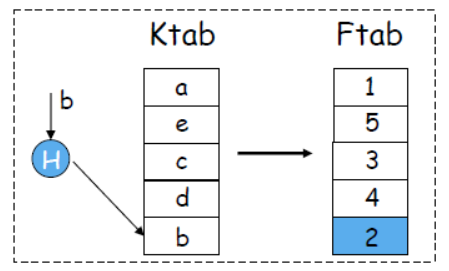
\includegraphics[width=0.4\linewidth]{pic/CP14/class descriptor}
    \caption{class descriptor}
\end{figure}

\subsection{Testing Class Membership}
Membership test: 为了安全的类型转换, 需要测试某个对象是否是某个类的实例. 

朴素(慢)的做法: 递归地检查 $x$ 的 class descriptor (记作 $x.0$) 开始的继承链, $\dots$ 如果发现某个是 $C$ 的 class descriptor 则 $x$ 是 $C$ 的实例; 否则如果到最上层仍未发现, 则说明不是 $C$ 的实例. 


更快的做法: display. 每个 class descriptor 储存一个 display, 也就是一个足够长(比最长继承链长)的定长列表, 记录对象的整条继承链. 就像: 
\begin{minted}{text}
    0: Object
    1: GrandparentClass
    2: ParentClass
    3: MeClass
    4: (nil)
    5: (nil)
    ...
\end{minted}
我们可以给每个类一个专属的数字 ID (例如对于 SI, 可以按照继承关系树的 BFS 序为每个类编号), 然后 display 中储存这些 ID 代表类. 由于对每个类, 其继承关系的嵌套深度在编译期已知, 因此可以立刻找到需要比较 display 中的哪一项. 例如, 假设 MeClass 的继承深度是第 3 层, 要检查 $x$ 是否为MeClass的实例, 只需检查 $x$ 的继承深度是否大于等于 3, 且 $x.0.display[3]$ 是否指向 MeClass 的 class descriptor 即可. 

\subsection{Private Fields and Methods}
private field/method: 私有的 field/method 只能被类的其他 method 访问/调用, 而不能被外部调用. 这是封装思想的体现: 调用者不该知道内部实现细节. 通过类型检查确保私密性(privacy): 每个访问/调用处检查是否 private.

